\section[IAM - Identity and Access Management]{\textbf{IAM - Identity and Access Management} \\ \textit{IAM - Định danh và quản lý quyền hạn}}

\subsection[Users \& Groups]{Users \& Groups}

\begin{itemize}
	\item IAM = Identity and Access Management, Global service 
	\item \textbf{Root account} created by default, shouldn't be used or shared  
	\item \textbf{Users} are people within your organization, and can be grouped
	\item \textbf{Group} only contain users, not other groups
	\item Users don't have to belong to a group,and user can belong to multiple groups (Người dùng không bắt buộc phải thuộc vào một nhóm nào, và một người dùng có thể thuộc về nhiều nhóm.)
\end{itemize}

\begin{figure}[htbp]
	\centering
	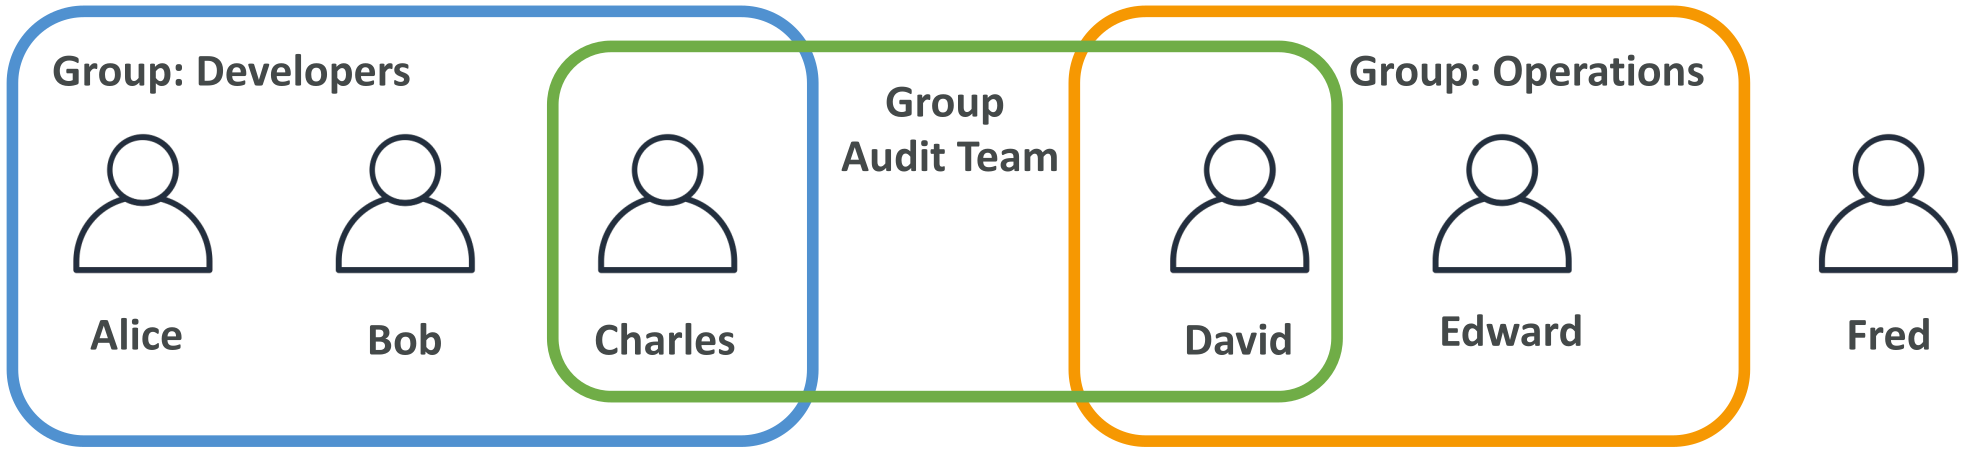
\includegraphics[width=0.8\textwidth]{images/iam-group}
	\caption{iam-group}
	\label{fig:iam-group}
\end{figure}

\subsection[Permissions]{Permissions \\ \textit{Các quyền hạn}}

\begin{itemize}
	\item \textbf{Users or Group} can be assigned JSON documents called policies (Các người dùng và nhóm có thể được gán tài liệu JSON được gọi là policies)
	\item These policies define the permission of the users (Các policies định nghĩa quyền hạn của các người dùng)
	\item In AWS you apply the \textbf{least privilege principle:} don't give more permissions than a user needs (Trong AWS, bạn áp dụng nguyên tắc đặc quyền tối thiểu: không cấp nhiều quyền hơn mức người dùng thực sự cần.)
\end{itemize}

\begin{figure}[htbp]
	\centering
	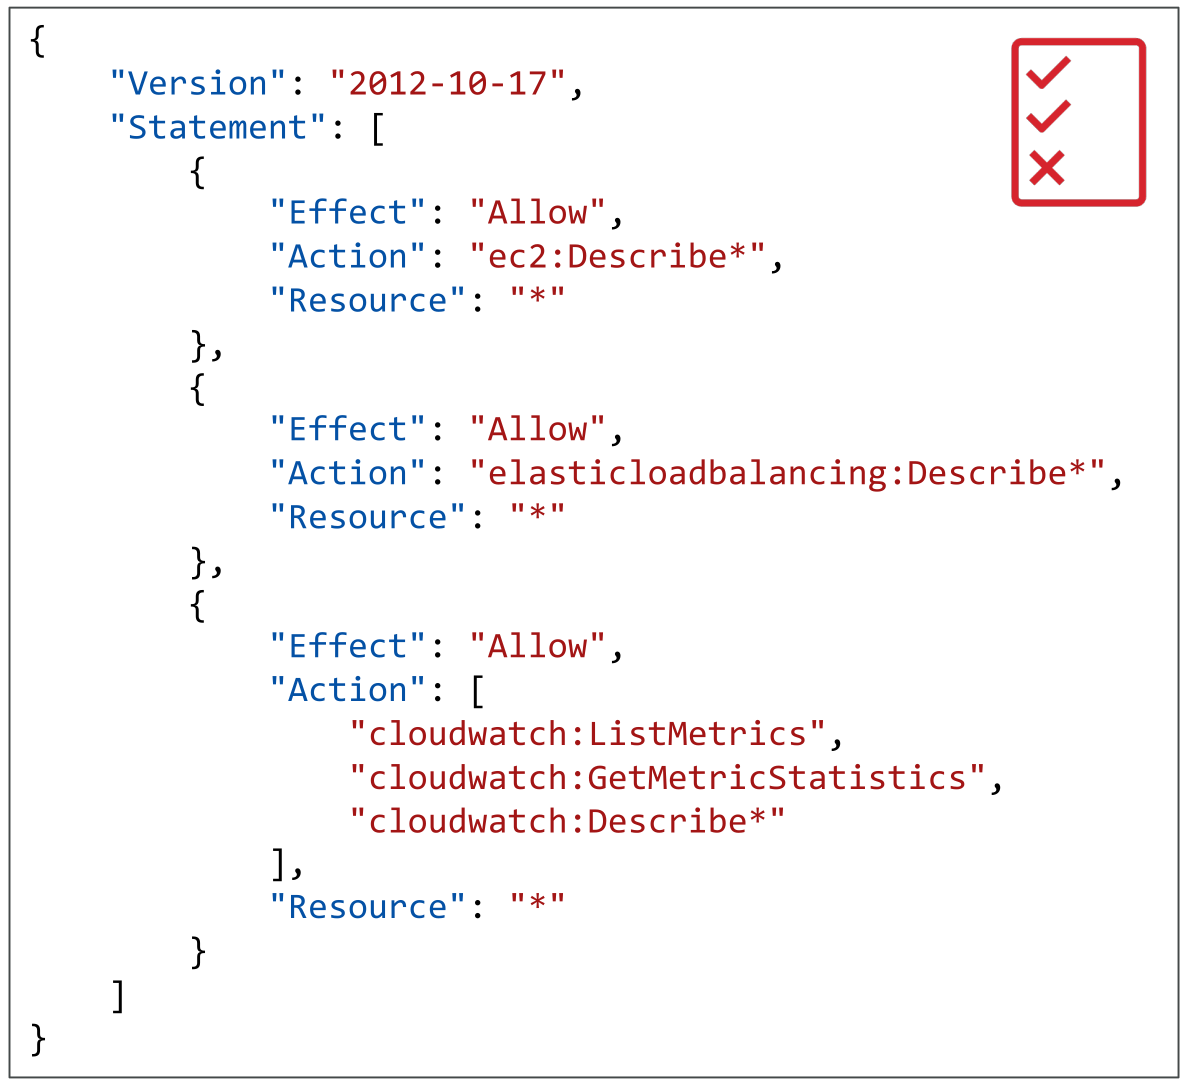
\includegraphics[width=0.2\textwidth]{images/iam-policies}
	\caption{iam-policies}
	\label{fig:iam-policies}
\end{figure}

\subsection[IAM Policies inheritance]{IAM Policies inheritance \\ \textit{Kế thừa IAM Policies}}

\begin{figure}[htbp]
	\centering
	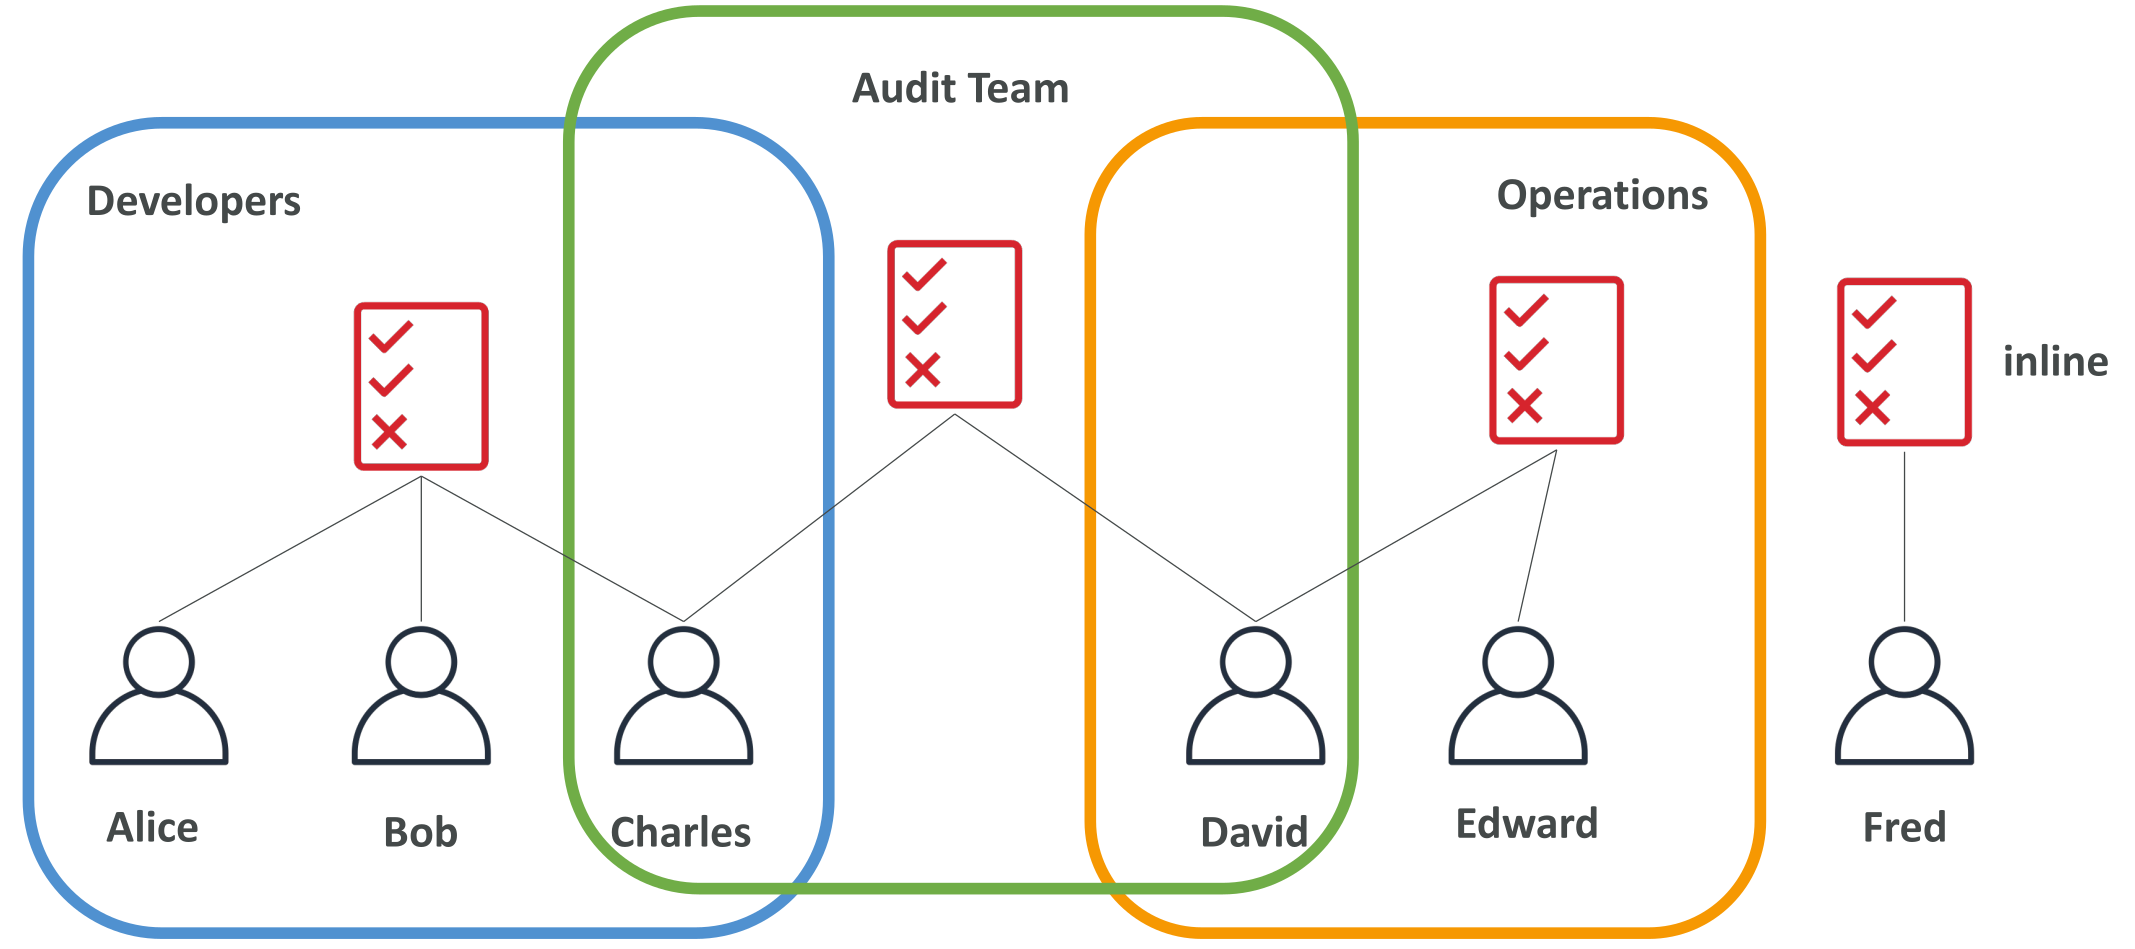
\includegraphics[width=0.8\textwidth]{images/iam-policies-inheritance}
	\caption{iam-policies-inheritance}
	\label{fig:iam-policies-inheritance}
\end{figure}

\subsection[IAM Policies structure]{IAM Policies structure \\ \textit{Cấu trúc IAM Policies}}

\begin{itemize}
	\item Consists of
	\begin{itemize}
		\item Version: policy language version, always include "2012-10-17"
		\item ID: an identifier for the policy (optional)
		\item Statement: one or more individual statements (required) (Một hoặc nhiều câu lệnh riêng lẻ)
	\end{itemize}
	\item Statement consists of
	\begin{itemize}
		\item Sid: an identifier for that statement (optional)
		\item Effect: whether the statement allows or denies access (Allow, Deny)
		\item Principal: account/ user/ role to which this policy applied to 
		\item Action: list of actions this policy allows or denies
		\item Resource: list of resources to which the actions applied to
		\item Condition: conditions for when this policy is in effect (optional)
	\end{itemize}
\end{itemize}

\begin{figure}[htbp]
	\centering
	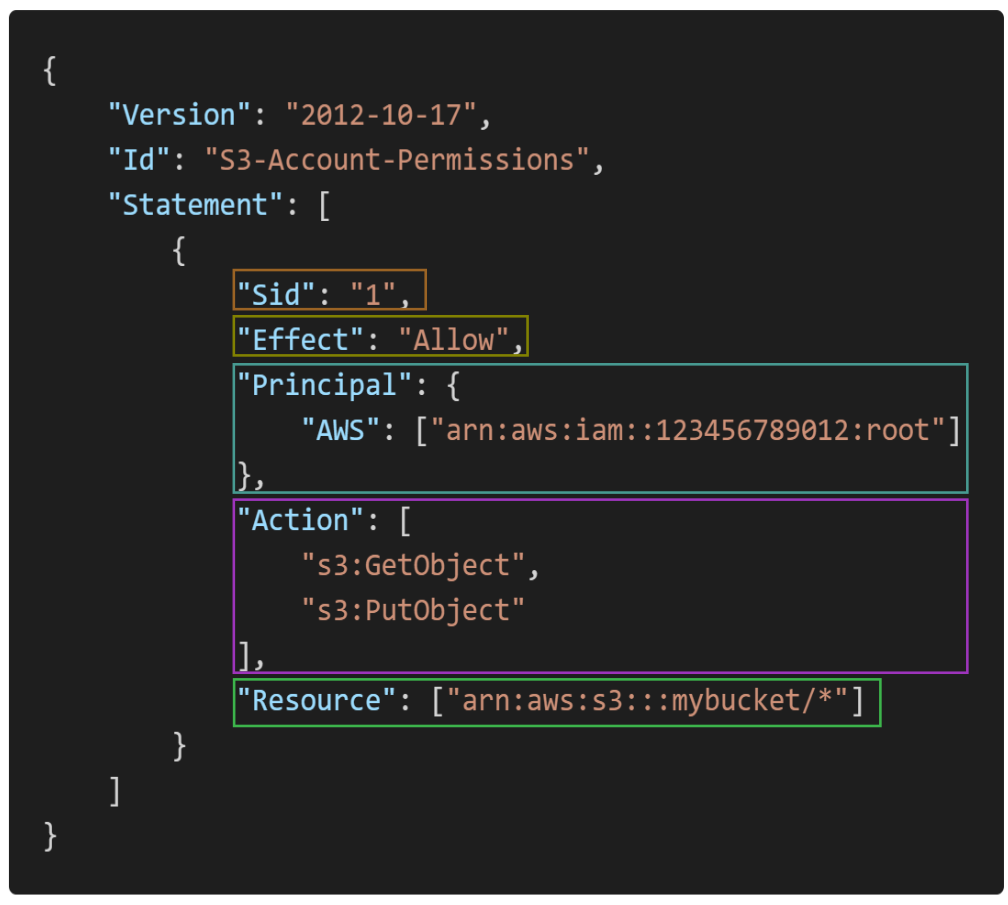
\includegraphics[width=0.2\textwidth]{images/iam-policies-structure}
	\caption{iam-policies-structure}
	\label{fig:iam-policies-structure}
\end{figure}


\subsection[IAM Password Policy]{IAM Password Policy \\ \textit{IAM chính sách mật khẩu}}

\begin{itemize}
	\item Strong passwords = higher security for your account
	\item In AWS, you can setup a password policy:
	\begin{itemize}
		\item Set a minimum password length
		\item Require specific character types:
		\begin{itemize}
			\item including uppercase letters
			\item lowercase letters
			\item numbers
			\item non-alphanumberic characters(Các ký tự không phải chữ cái và số)
		\end{itemize}
		\item Allow all IAM users to change their own passwords
		\item Require users to change their password after some time (password expiration)
		\item Prevent password re-user
	\end{itemize}
\end{itemize}


\subsection[Multi Factor Authentication - MFA]{Multi Factor Authentication - MFA \\ \textit{Nhiều tác nhân Xác thực}}

\begin{itemize}
	\item Users have access to your account and can possibly change configurations or delete resources in your AWS account 
	\item You want to protect your Root Accounts and IAM users
	\item MFA = password you know + security device you own
	\item Main benefit of MFA: if a password is stolen or hacked, the account is not compromised (Nếu mật khẩu bị đánh cắp hoặc bị hack, tài khoản của bản không bị xâm nhập)
\end{itemize}
	\begin{figure}[htbp]
		\centering
		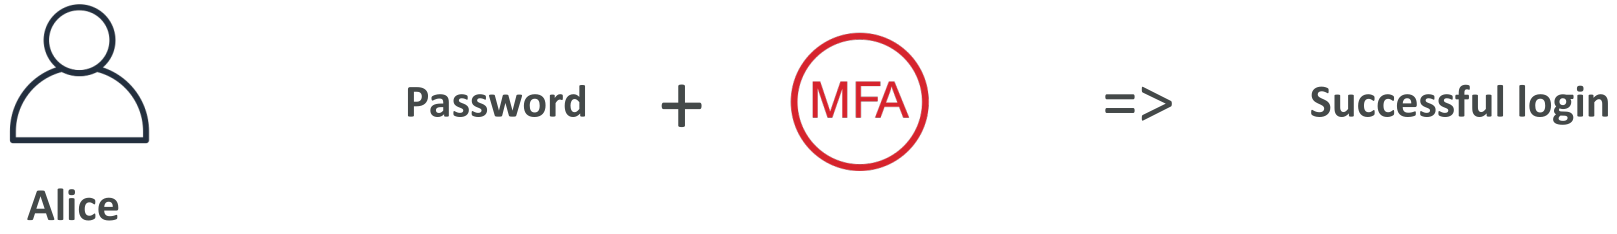
\includegraphics[width=0.8\textwidth]{images/iam-password-mfa}
		\caption{iam-password-mfa}
		\label{fig:iam-password-mfa}
	\end{figure}

\newpage

\subsection[MFA devices options in AWS]{MFA devices options in AWS \\ \textit{Tùy chọn thiết bị MFA trong AWS}}


\begin{figure}[htbp]
	\centering
	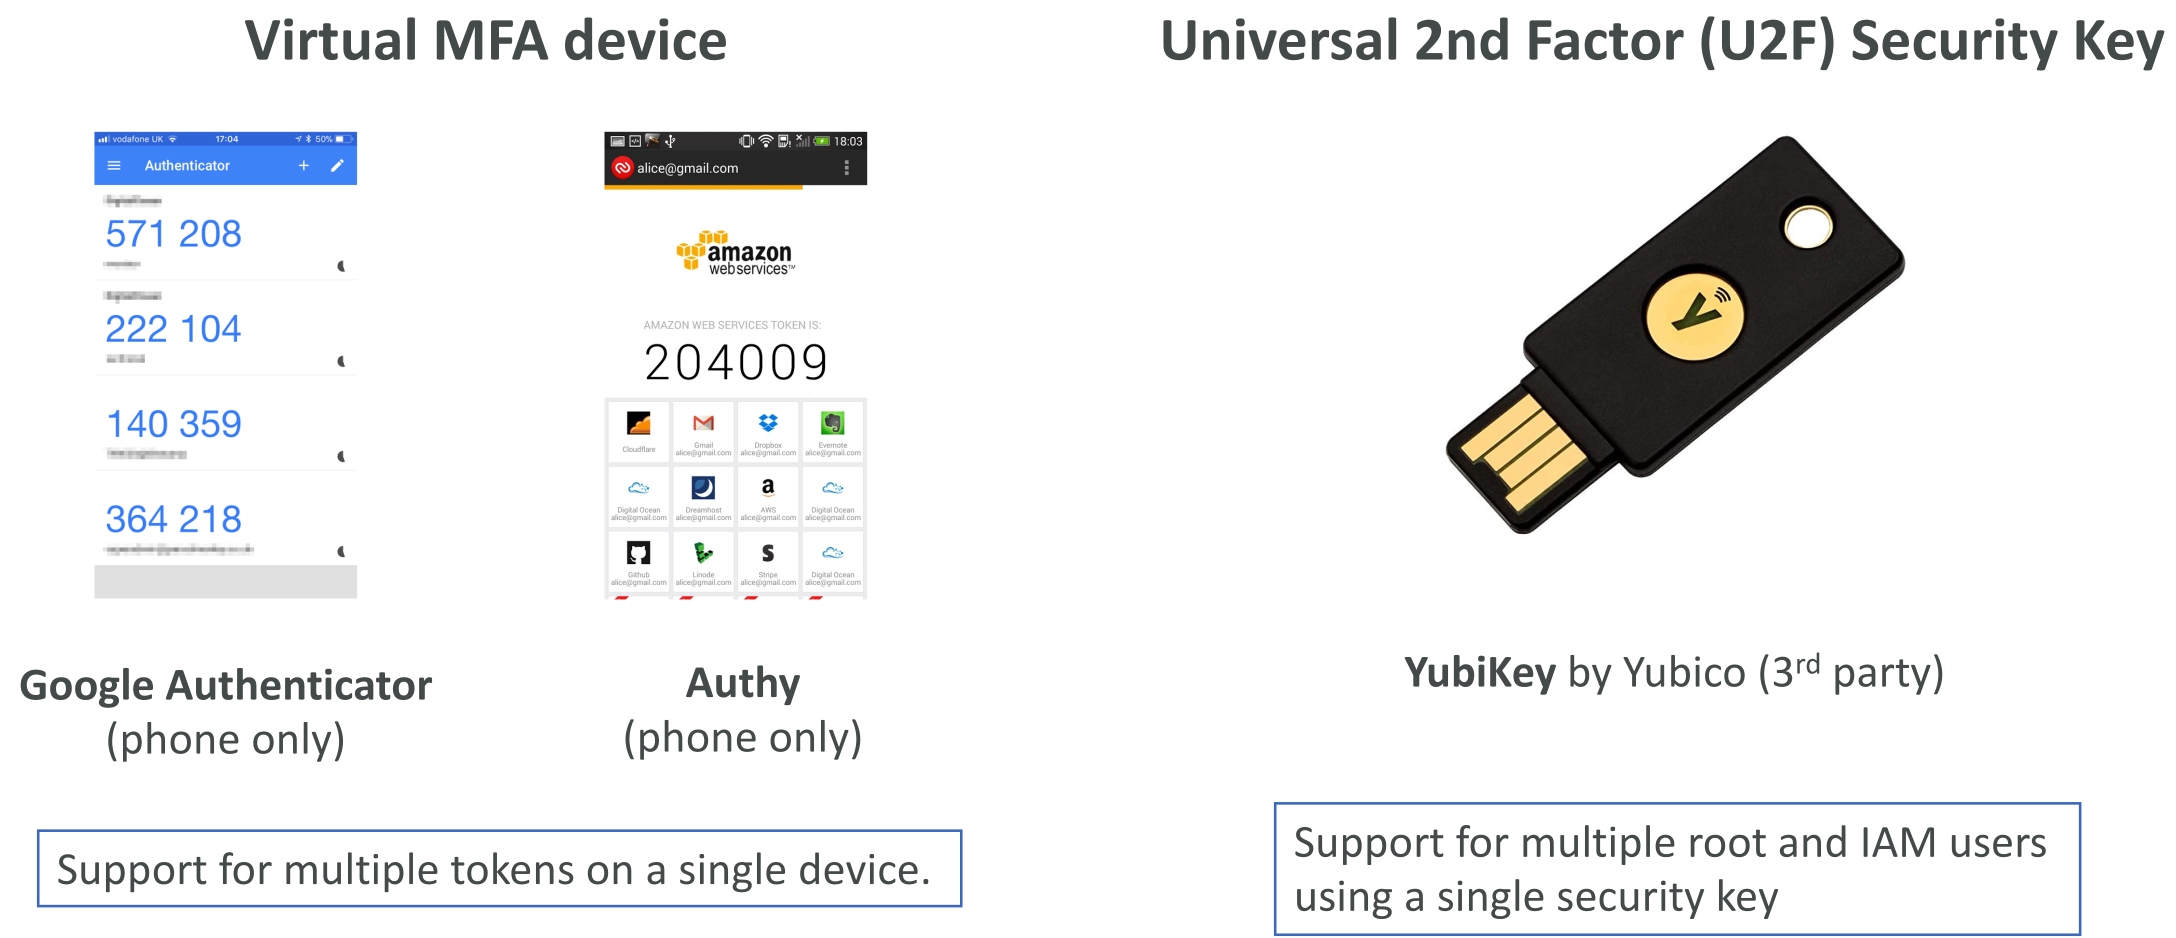
\includegraphics[width=0.8\textwidth]{images/iam-mfa-option-devices}
		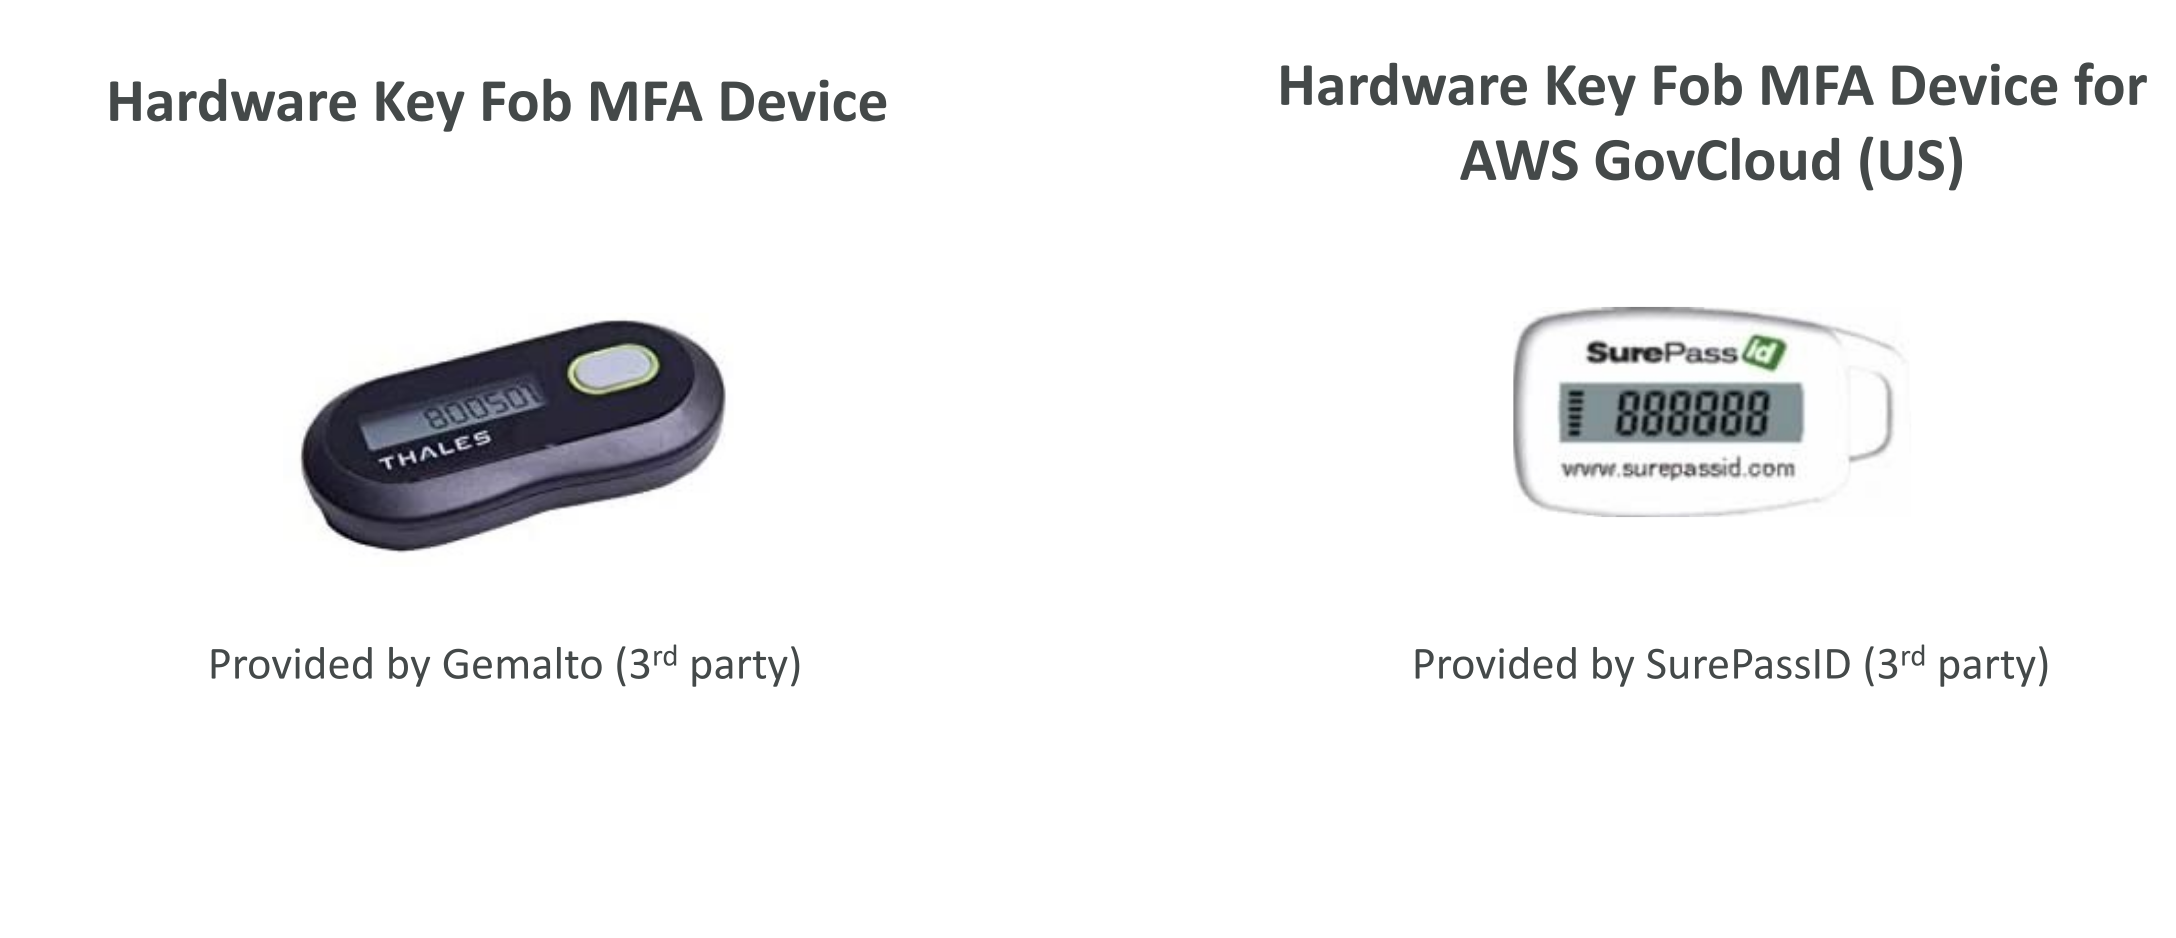
\includegraphics[width=0.8\textwidth]{images/iam-mfa-option-devices-02}
	\caption{iam-mfa-option-devices}
	\label{fig:iam-mfa-option-devices}
\end{figure}

\subsection[How can users access AWS?]{How can users access AWS? \\ \textit{Người dùng truy cập AWS bằng cách nào?}}

\begin{itemize}
	\item To access AWS, you have three options:
	\begin{itemize}
		\item AWS Management Console (protected by password + MFA)
		\item AWS Command Line Interface (CLI): protected by access keys
		\item AWS Software Developer Kit (SDK) - for code: protected by access keys
	\end{itemize}
	\item Access Key are generated through the AWS Console (Access Key được tạo thông qua bảng điều khiển của AWS)
	\item Users manage their own access keys
	\item Access Keys are secret, just like a password. Don't share them
	\item Access Key ID ~= username
	\item Secret Access Key ~= password
\end{itemize}


\subsection[What’s the AWS CLI?]{What’s the AWS CLI? \\ \textit{AWS CLI là gì?}}

\begin{itemize}
	\item A tool that enables you to interact with AWS services using commands in your command-line shell (Một công cụ cho phép bạn tương tác với các dịch vụ aws bằng cách sử dụng các dòng lệnh trong command-line shell của bạn)
	\item Direct access to the public APIs of AWS services(Truy cập trực tiếp đến các API công khai của các dịch vụ AWS)
	\item You can develop scripts to manage your resources 
	\item It’s open-source: \url{https://github.com/aws/aws-cli}
	\item Alternative to using AWS Management Console (Phương án thay thế cho việc sử dụng AWS Management Console)
\end{itemize}


\subsection[What’s the AWS SDK?]{What’s the AWS SDK? \\ \textit{SDK CLI là gì?}}

\begin{itemize}
	\item AWS Software Development Kit (AWS SDK)
	\item Language-specific APIs (set of libraries)(Các API dành riêng cho từng ngôn ngữ lập trình (tập hợp các thư viện))
	\item Enables you to access and manage AWS services   programmatically (Cho phép truy cập và quản lý các dịch vụ AWS bằng lập trình)
	\item Embedded within your application (Được nhúng bên trong ứng dụng của bạn)
	\item Supports
	\begin{itemize}
		\item SDKs (JavaScript, Python, PHP, .NET, Ruby, Java, Go, Node.js,
		C++)
		\item Mobile SDKs (Android, iOS, …)
		\item IoT Device SDKs (Embedded C, Arduino, …)
	\end{itemize}
	\item Example: AWS CLI is built on AWS SDK for Python 
\end{itemize}

\subsection[IAM Roles for Services]{IAM Roles for Services \\ \textit{IAM Roles cho các dịch vụ}}

\begin{itemize}
	\item Some AWS service will need to perform actions on your behalf (Một vài dịch vụ AWS cần thực hiện các hoạt động thay mặt bạn)
	\item To do so, we will assign permissions to AWS services with IAM Roles(Để làm được điều đó, chúng ta sẽ gán quyền cho các dịch vụ AWS thông qua IAM Roles.)
	\item Common roles (các vai trò phổ biến):
	\begin{itemize}
		\item EC2 Instance Roles
		\item Lambda Function Roles
		\item Roles for CloudFormation
	\end{itemize}
\end{itemize}

\begin{figure}[htbp]
	\centering
	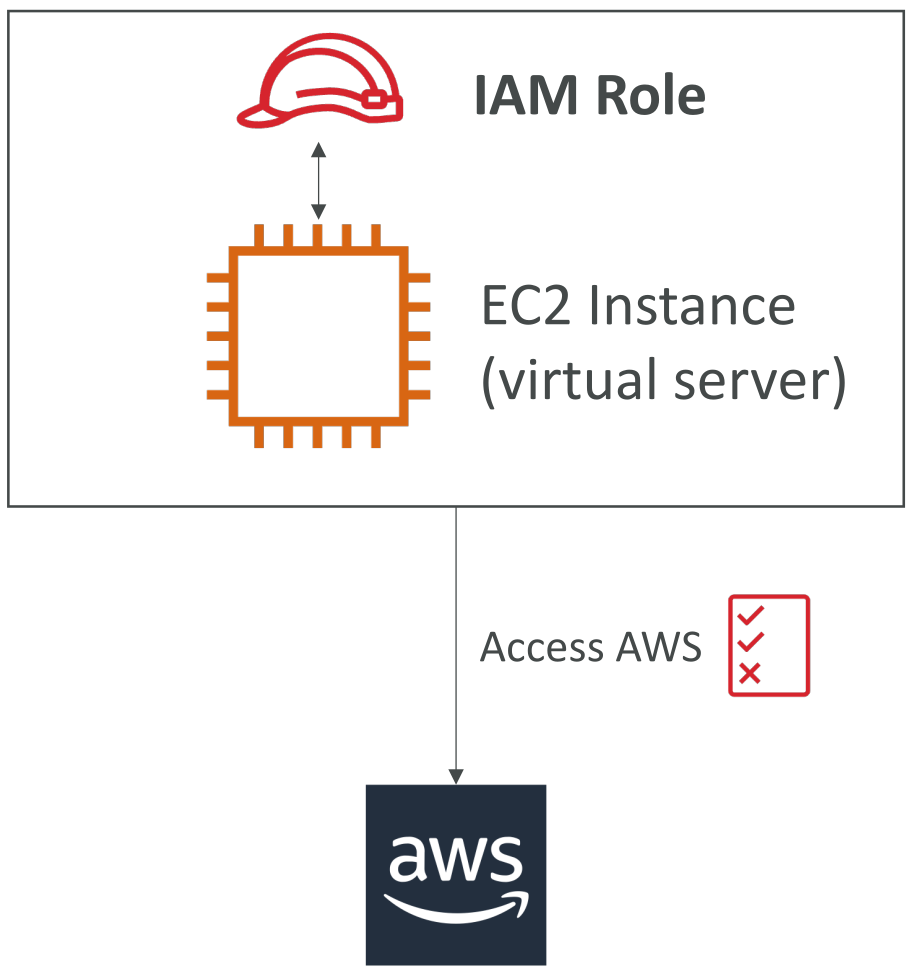
\includegraphics[width=0.5\textwidth]{images/iam-roles}
	\caption{iam-roles}
	\label{fig:iam-roles}
\end{figure}

\subsection[IAM Security Tools]{IAM Security Tools \\ \textit{Các công cụ bảo mật IAM}}

\begin{itemize}
	\item IAM Credentials Report (account-level)
	\begin{itemize}
		\item A report that lists all your account's users and the status of their various credentials (Báo cáo liệt kê tất cả người dùng trong tài khoản của bạn và trạng thái của các loại thông tin xác thực mà họ đang sử dụng)
	\end{itemize}
	\item IAM Access Advisor (user-level)
	\begin{itemize}
		\item Access Advisor shows the service permissions granted to a user and when those services were last accessed (Access Advisor cho thấy các quyền truy cập dịch vụ đã được cấp cho một người dùng và thời điểm các dịch vụ đó được truy cập lần cuối)
		\item You can use this information to revise your policies (Bạn có thể sử dụng các thông tin này để sửa đổi các policy của bạn)
	\end{itemize}
\end{itemize}

\subsection[IAM Guidelines \& Best Practies]{IAM Guidelines \& Best Practies \\ \textit{IAM Hướng dẫn và cách làm tối ưu nhất}}

\begin{itemize}
	\item Don't use the root account except for AWS account setup (Chỉ sử dụng tài khoản root cho các bước thiết lập ban đầu của tài khoản AWS.)
	\item One physical user = One AWS user (Mỗi người dùng thực tế nên có một tài khoản người dùng AWS riêng biệt)
	\item Assign users to groups and assign permissions to groups
	\item Create a strong password policy
	\item Use and enforce the use of Multi Factor Authentication (MFA)
	\item Create and use Roles for giving permissions to AWS services 
	\item Use Access Keys for Programmatic Access (CLI/SDK)
	\item Audit permissions of your account using IAM Credentials Report \& IAM Access Advisor (Kiểm tra quyền truy cập của tài khoản của bạn bằng cách sử dụng IAM Credentials Report và IAM Access Advisor)
	\item Never share IAM users \& Access Keys
\end{itemize}



\subsection[Shared Responsibility Model for IAM]{Shared Responsibility Model for IAM \\ \textit{Mô hình chia sẻ trách nhiệm của IAM}}

\begin{itemize}
	\item AWS
	\begin{itemize}
		\item Infrastructure (global network security)
		\item Configuration and vulnerability analysis (Cấu hình và phân tích lỗ hổng bảo mật)
		\item Compliance validation  (Xác thực tuân thủ)
	\end{itemize}
	\item You
	\begin{itemize}
		\item Users, Groups, Roles, Policies
		management and monitoring (quản lý và giám sát)
		\item Enable MFA on all accounts
		\item Rotate all your keys often (Thường xuyên thay đổi các key của bạn)
		\item Use IAM tools to apply
		appropriate permissions (Sử dụng các công cụ IAM để áp dụng quyền hạn thích hợp)
		\item Analyze access patterns \& review permission (Phân tích các mẫu truy cập và xem lại các quyền truy cập)
	\end{itemize}
\end{itemize}


\subsection[IAM - Summary]{IAM - Summary}

\begin{itemize}
	\item Users: mapped to a physical user, has a password for AWS Console (gắn liền với người dùng thât, có mật khẩu để đăng nhập AWS Console)
	\item Groups: contains users only
	\item Policies: JSON document that outlines permissions for users or groups (là tài liệu JSON mô tả các quyền truy cập dành cho người dùng hoặc nhóm.)
	\item Roles: for EC2 instances or AWS services
	\item Security: MFA + Password Policy
	\item AWS CLI: manage your AWS services using the command-line
	\item AWS SDK:manage your AWS services using a programming language 
	\item Access Keys: access AWS using the CLI or SDK
	\item Audit: IAM Credential Reports \& IAM Access Advisor
\end{itemize}














































